Figure \ref{fig:iaea-jendl-dnp-yield} shows the percentage of the total delayed neutron yield that comes from the six \glspl{DNP} with the largest yield contribution, where the yield from each \gls{DNP} is defined by Equation \eqref{eq:summation-tdny}.
This equation shows that the largest yield contributors have large emission probabilities $P_n$ and cumulative fission yields $CFY$.
This doesn't necessarily indicate there will be a large concentration of the \gls{DNP}, as it may be short lived, but rather for any given fission, that \gls{DNP} has a higher probability to form and emit a delayed neutron.
The total delayed neutron yield for this dataset is 0.0160 delayed neutrons per fission event.
There are a total of 220 \glspl{DNP} in this dataset, and five of them capture over 50\% of the total delayed neutron yield.

\begin{figure}
    \centering
    
\includegraphics[width=0.5\linewidth]{images/iaea/dnp_yield.png}
    \caption{The fraction of the delayed neutron yield from particular \glspl{DNP} from JENDL-5 cumulative fission yields and IAEA beta-delayed neutron emission database half-lives and emission probabilities. The five \glspl{DNP} with the largest delayed neutron yield contributions supply over 50\% of the total delayed neutrons per fission event. The remaining 215 \glspl{DNP} provide approximately 48\% of the total delayed neutron yield.}
    \label{fig:iaea-jendl-dnp-yield}
\end{figure}


Figure \ref{fig:count-rate-iaea-jendl} shows the histogram for the sampled group one half-lives $\tau_1$ as well as how the delayed neutron count rate compares to those using \gls{DNP} group parameters from the literature \cite{keepin1957delayed, brady1989delayed, synetos1983delayed}.
The histogram shows that the group parameters follow a normal distribution as the nuclear data for each \gls{DNP} is randomly sampled, with the group half-life as the mean of that normal distribution.
Although not shown, the other group parameters follow this same trend.
The Keepin normalized delayed neutron count rate shows how the delayed neutron count rate calculated in this work, both for every count rate from the sampled data and from the group fit using the calculated \gls{DNP} group parameters compare.
A value of 1 at any given time indicates the delayed neutron count rate at that time perfectly matches the delayed neutron count rate from the Keepin et al. \gls{DNP} group parameters.
These results show that the Keepin et al. \gls{DNP} group parameters agree well with group parameters calculated using the \gls{IAEA} beta-delayed neutron emission database and JENDL-5 cumulative fission yields, with differences smaller than those from Brady and England and from Synetos and Williams.

\begin{figure}[!ht]
\centering
\subfloat[The \gls{DNP} group one half-life $\tau_1$ evaluated based on the mean of the sampled data.]{
  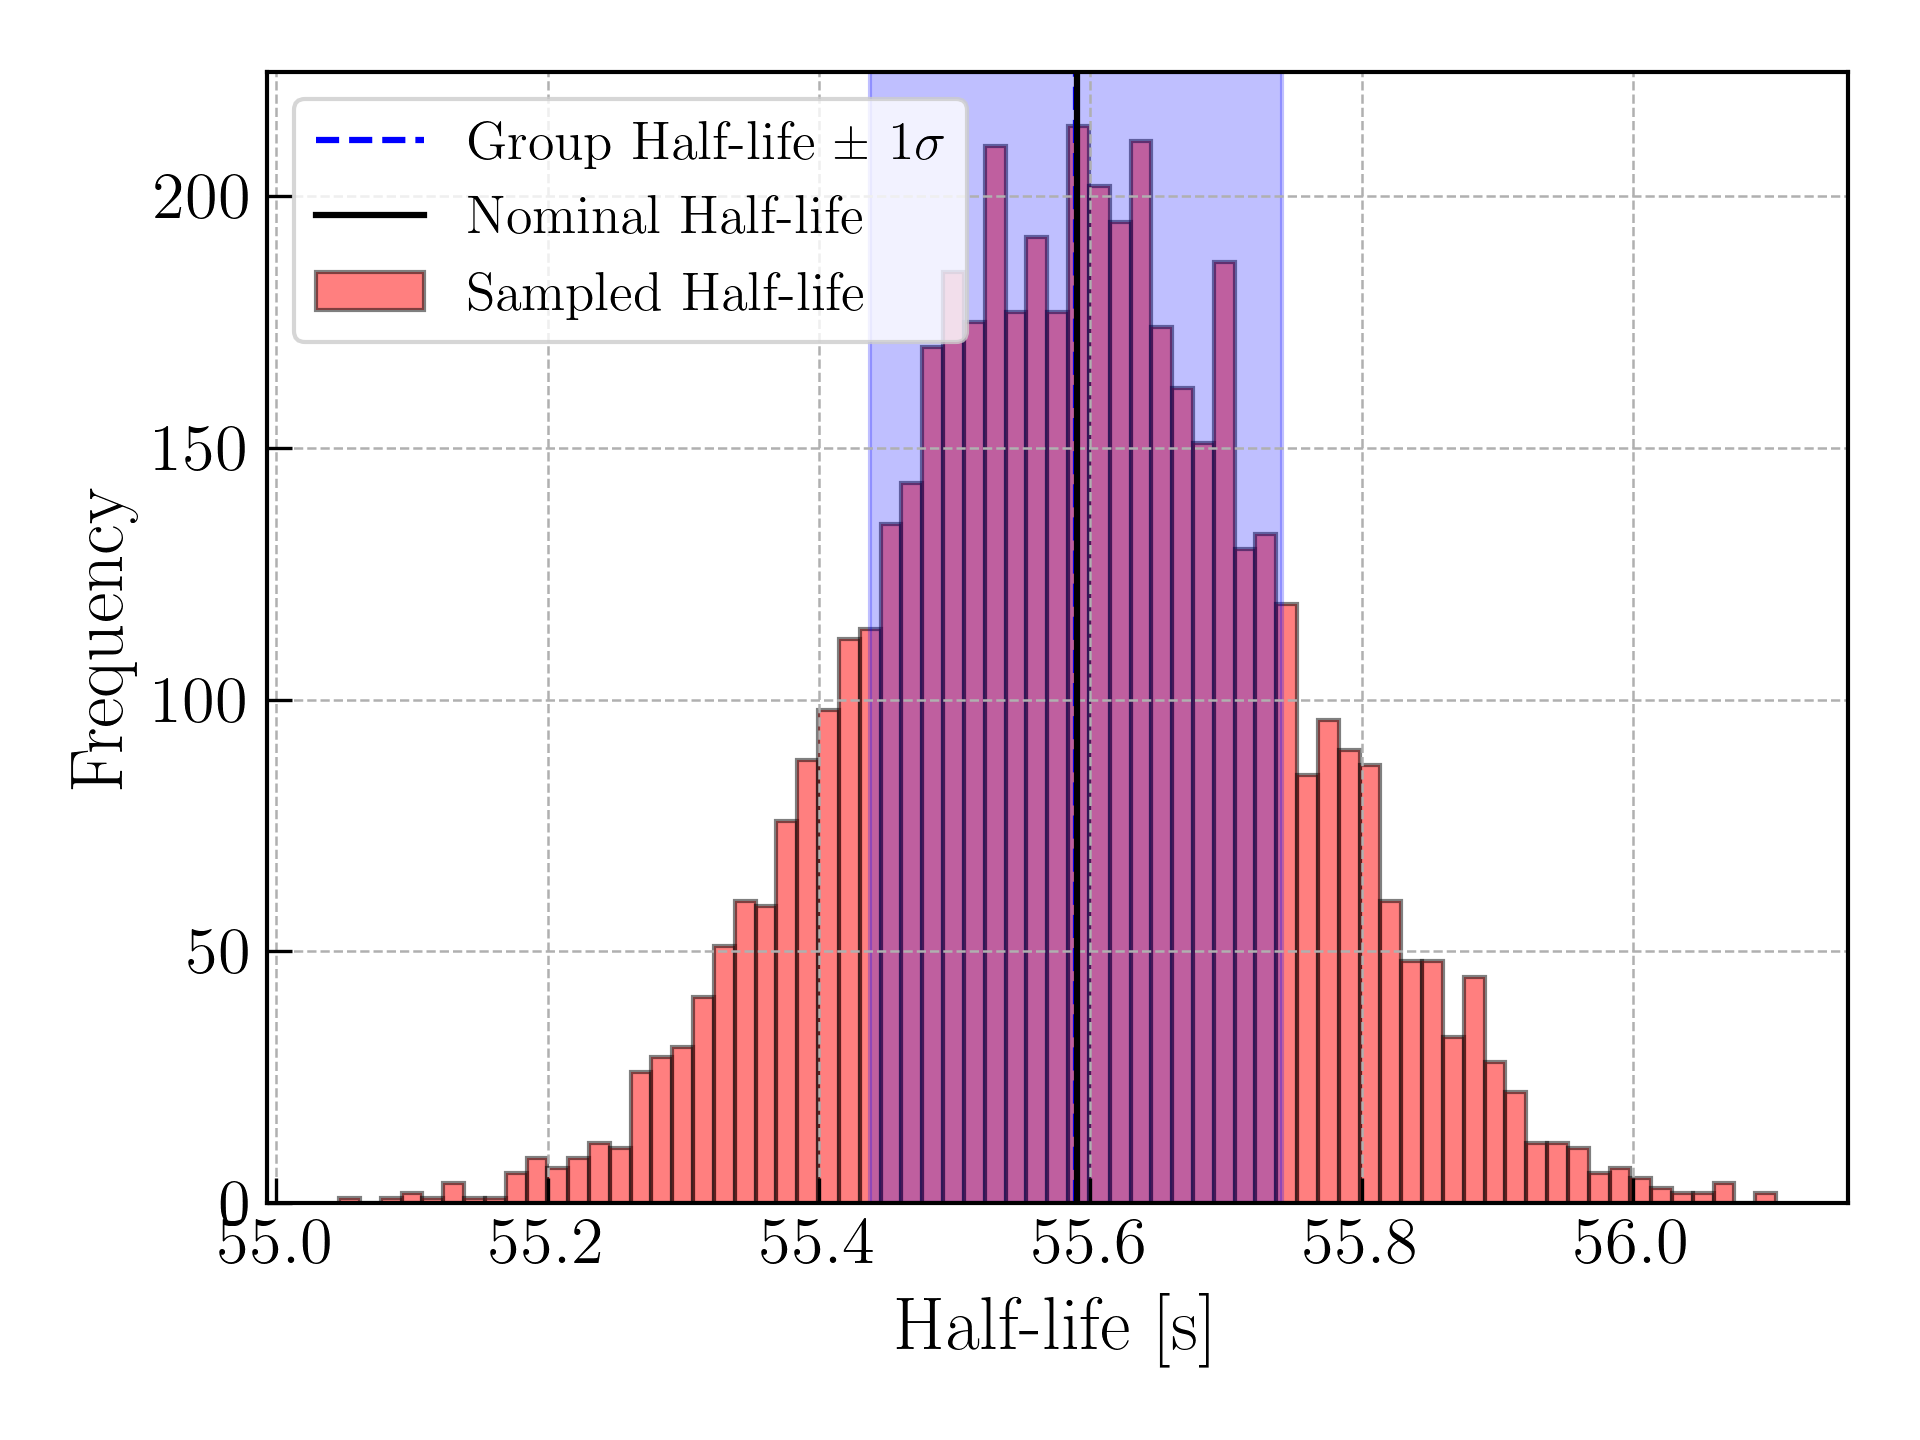
\includegraphics[width=0.45\linewidth]{images/iaea/MC_group1_half_life.png}
}
\hspace{0.05\linewidth}
\subfloat[The delayed neutron count rate as a function of time relative to the Keepin et al. \gls{DNP} group parameter delayed neutron count rate for \gls{DNP} six group parameters from this work, Brady and England, and Synetos and Williams \cite{keepin1957delayed, brady1989delayed, synetos1983delayed}.]{
  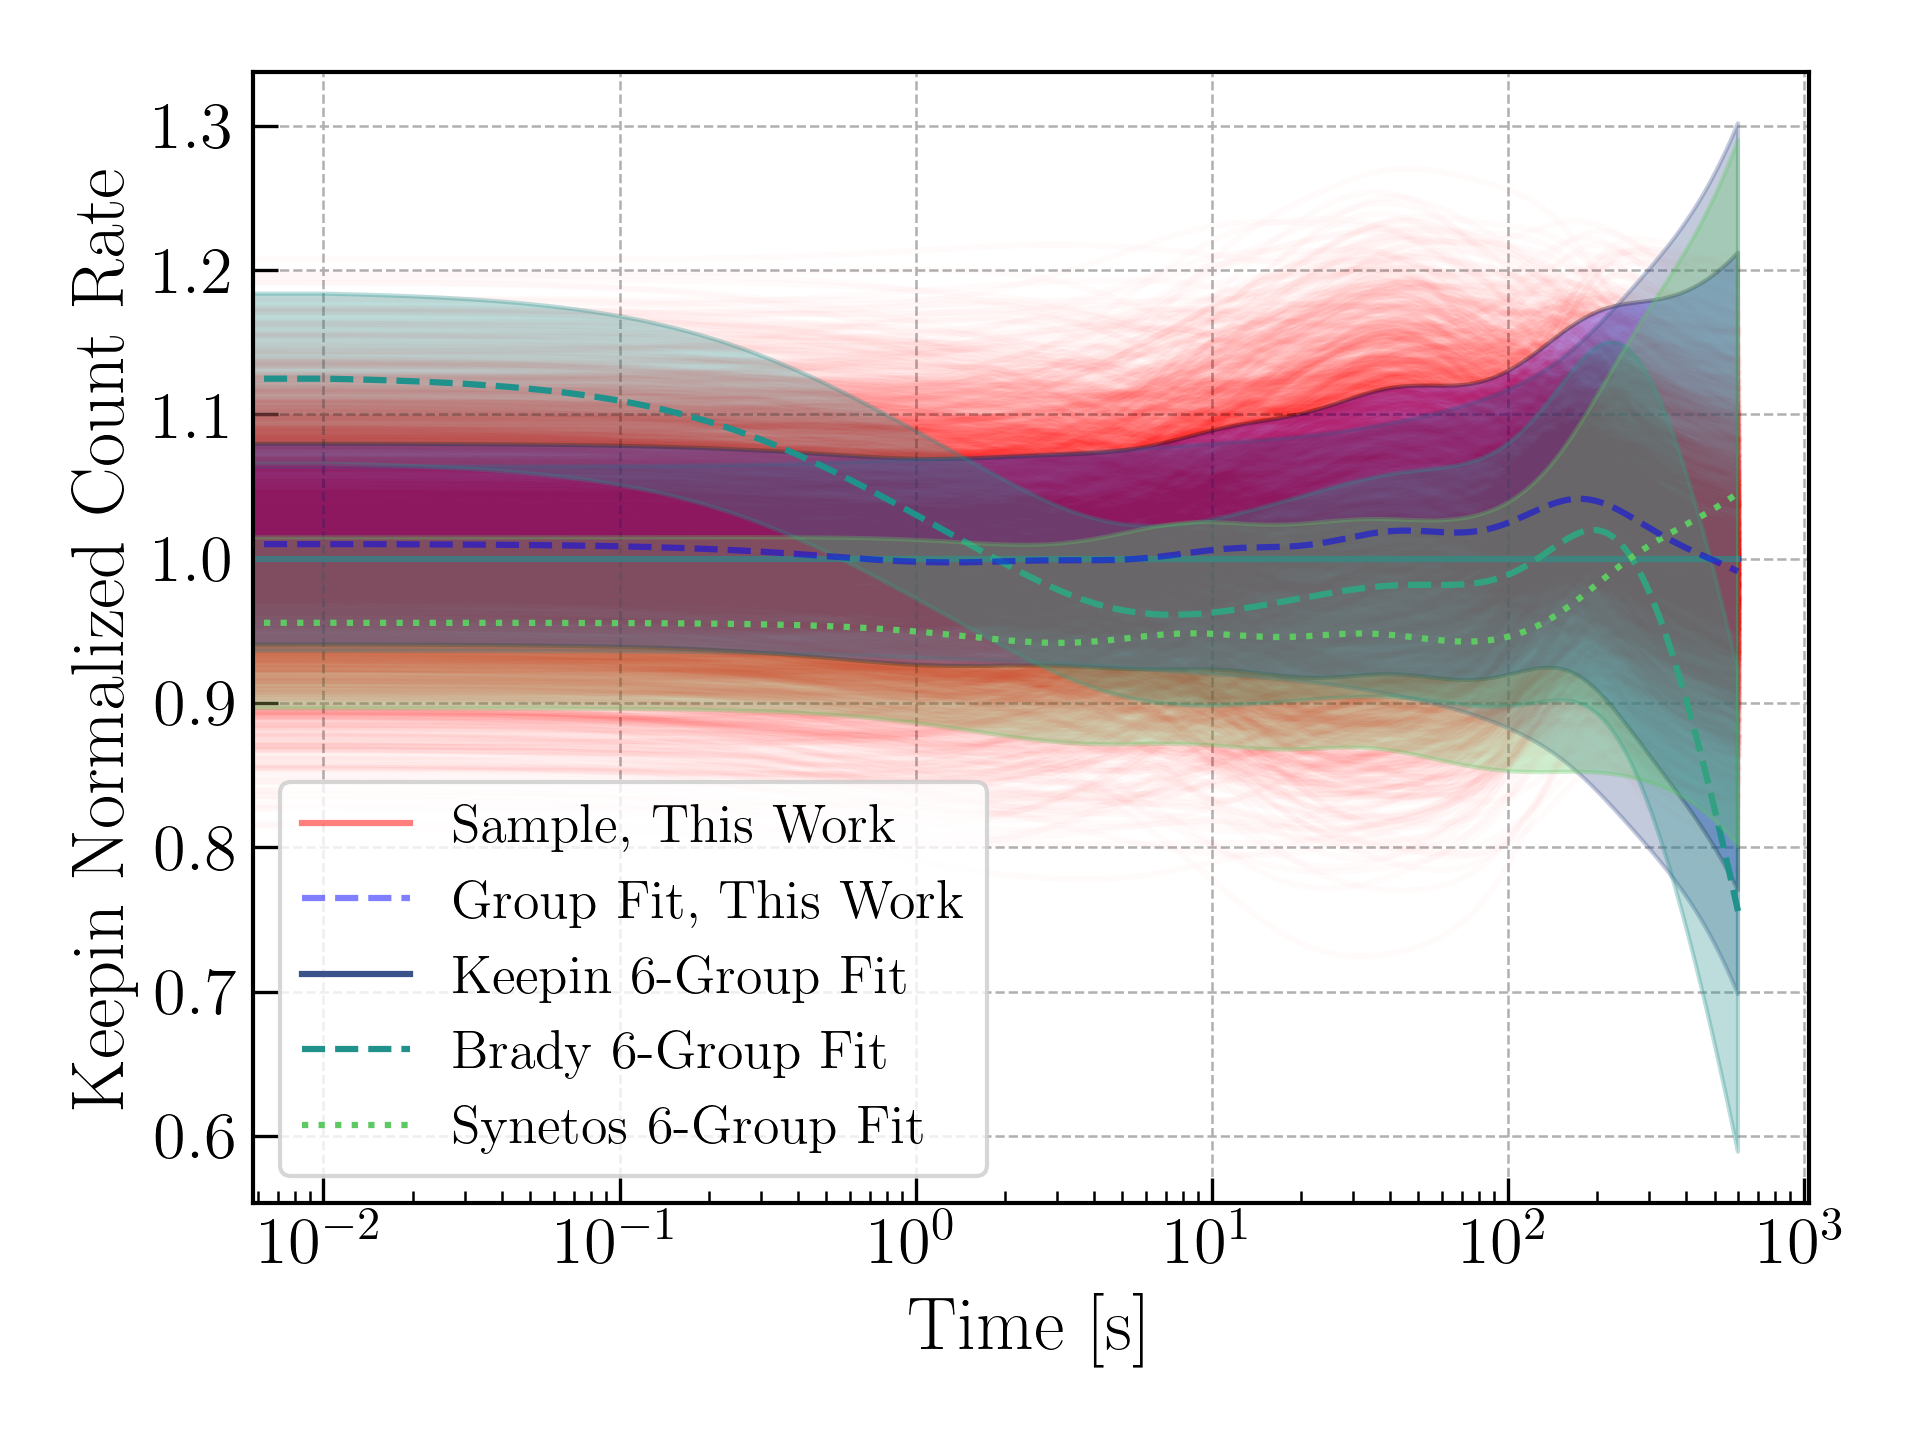
\includegraphics[width=0.45\linewidth]{images/iaea/Keepin_counts.png}
}
\caption{These plots show how the 5000 samples lead to a distribution of \gls{DNP} group parameters and delayed neutron count rates from JENDL-5 cumulative fission yields and IAEA beta-delayed neutron emission database half-lives and emission probabilities. The \gls{DNP} group one half-life $\tau_1$ shows a normal distribution about a mean, while the Keepin et al. normalized count rate shows this work offers good agreement with the literature.}
\label{fig:count-rate-iaea-jendl}
\end{figure}

Figure \ref{fig:sens-iaea-jendl} shows an example for how the \glspl{PCC} are calculated using the 5000 samples.
Each sample is represented as a single point at which the nuclear data is sampled from a normal distribution.
Specifically for this figure, the samples are plotted as a function of the $^{137}$I half-life.
Figure \ref{fig:sens-iaea-jendl}(a) shows how the group one \gls{DNP} half-life $\tau_1$ changes as a function of the $^{137}$I half-life.
There is no clear increase or decrease in the group one half-life as the $^{137}$I half-life varies, which is why the \gls{PCC} is 0.005 for that combination.
However, Figure \ref{fig:sens-iaea-jendl}(b) shows how the group two \gls{DNP} half-life $\tau_2$ has a much stronger correlation, resulting in a \gls{PCC} of 0.73.
These \gls{PCC} values are calculated for the emission probability, concentration, and half-life for each group for each \gls{DNP}.

\begin{figure}[!ht]
\centering
\subfloat[The relative change in the group one half-life $\tau_1$ due to relative change in the $^{137}$I half-life with a \gls{PCC} of 0.005.]{
  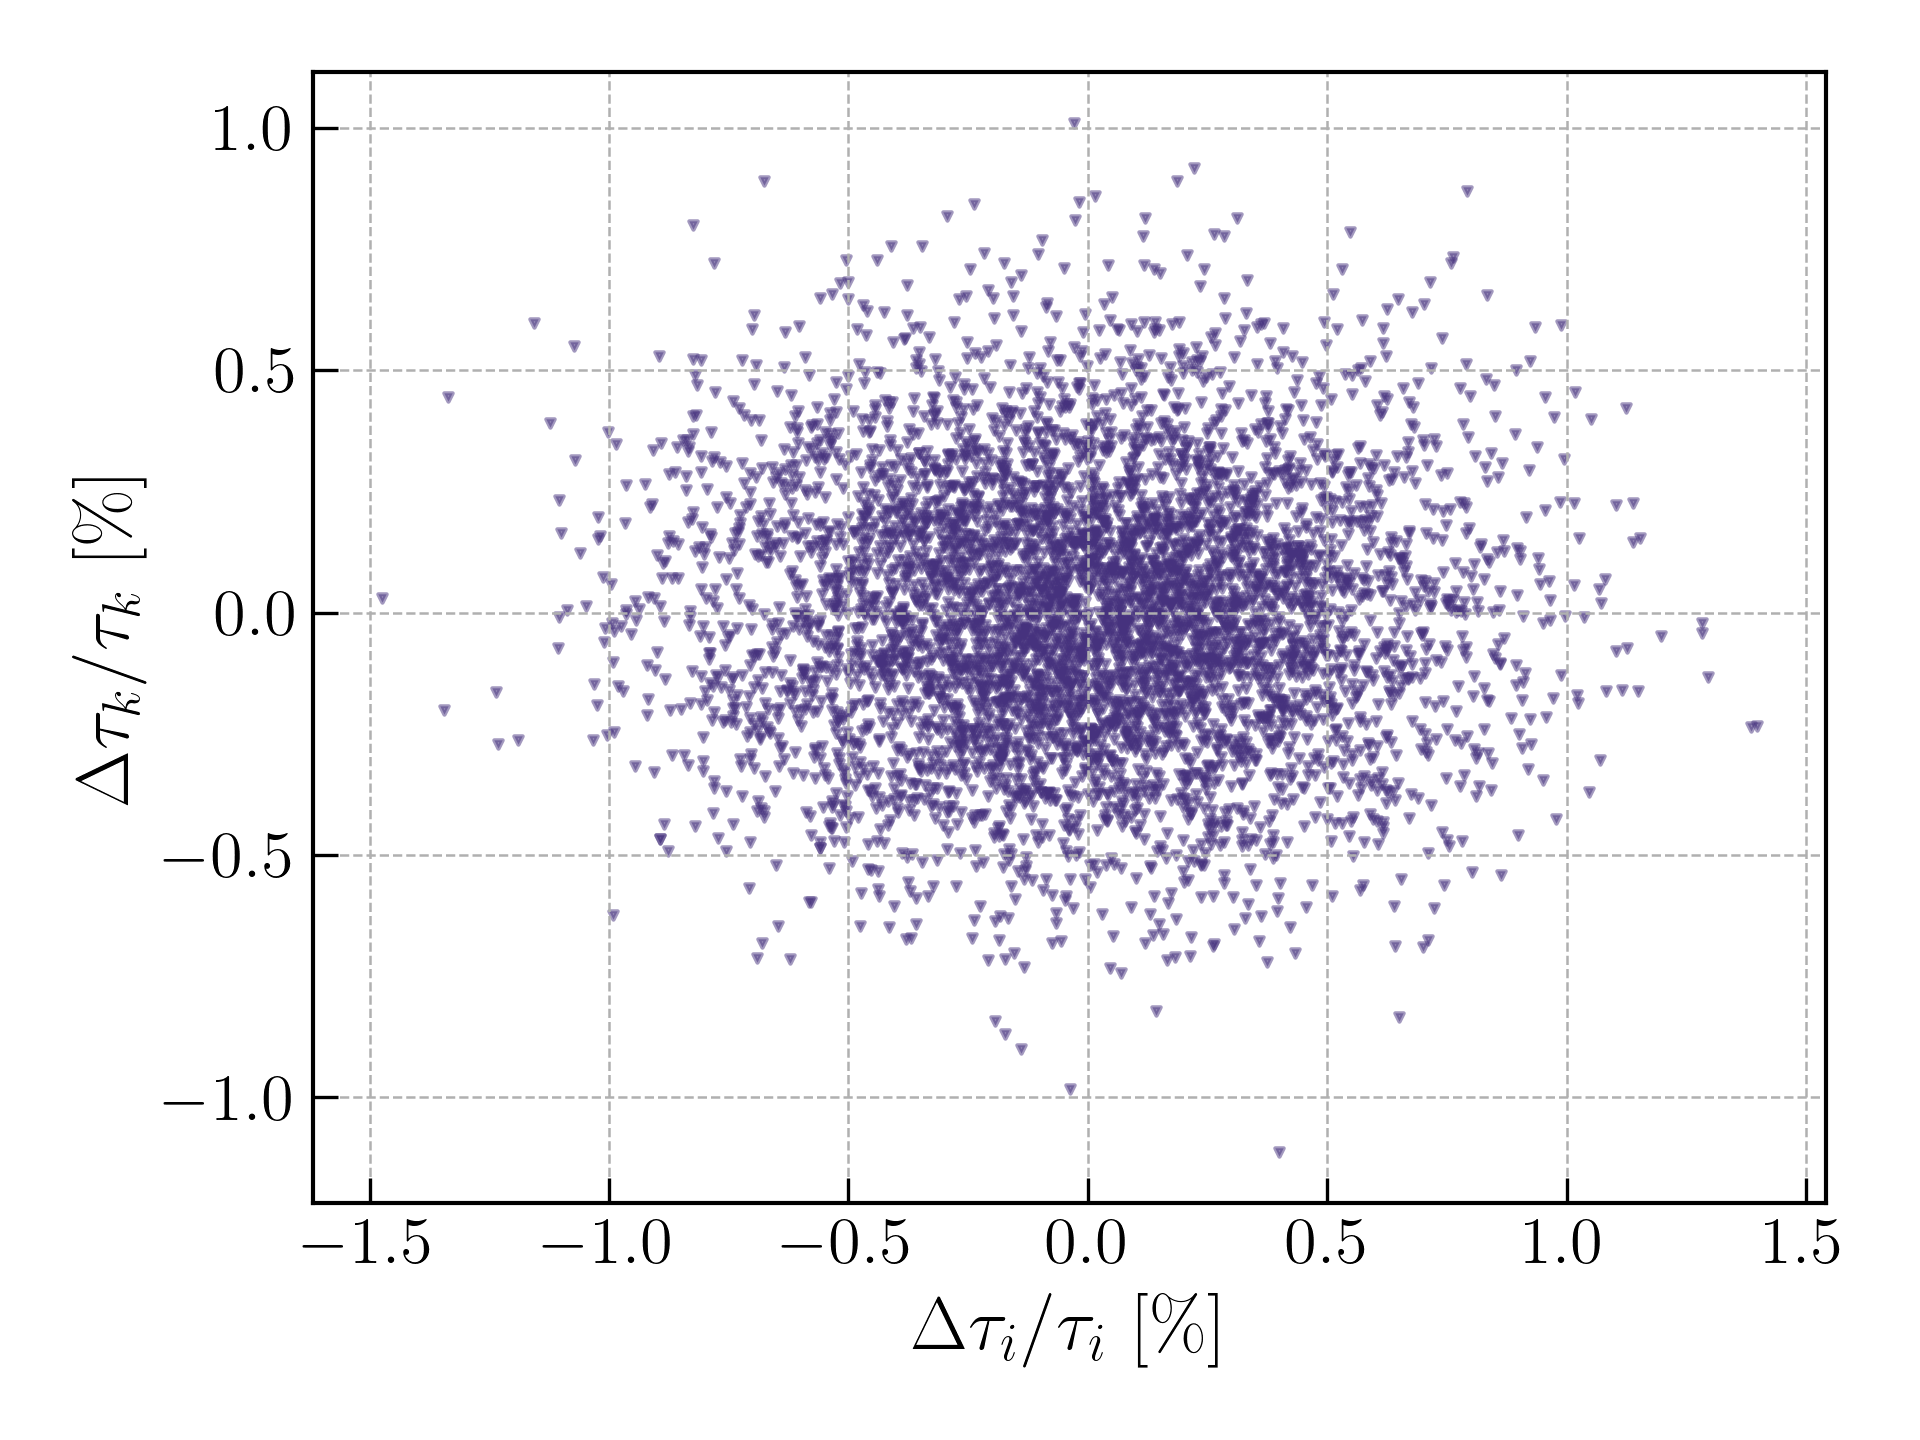
\includegraphics[width=0.45\linewidth]{images/iaea/sens_lam_halflife_I137_1.png}
}
\hspace{0.05\linewidth}
\subfloat[The relative change in the group two half-life $\tau_2$ due to relative change in the $^{137}$I half-life with a \gls{PCC} of 0.726.]{
  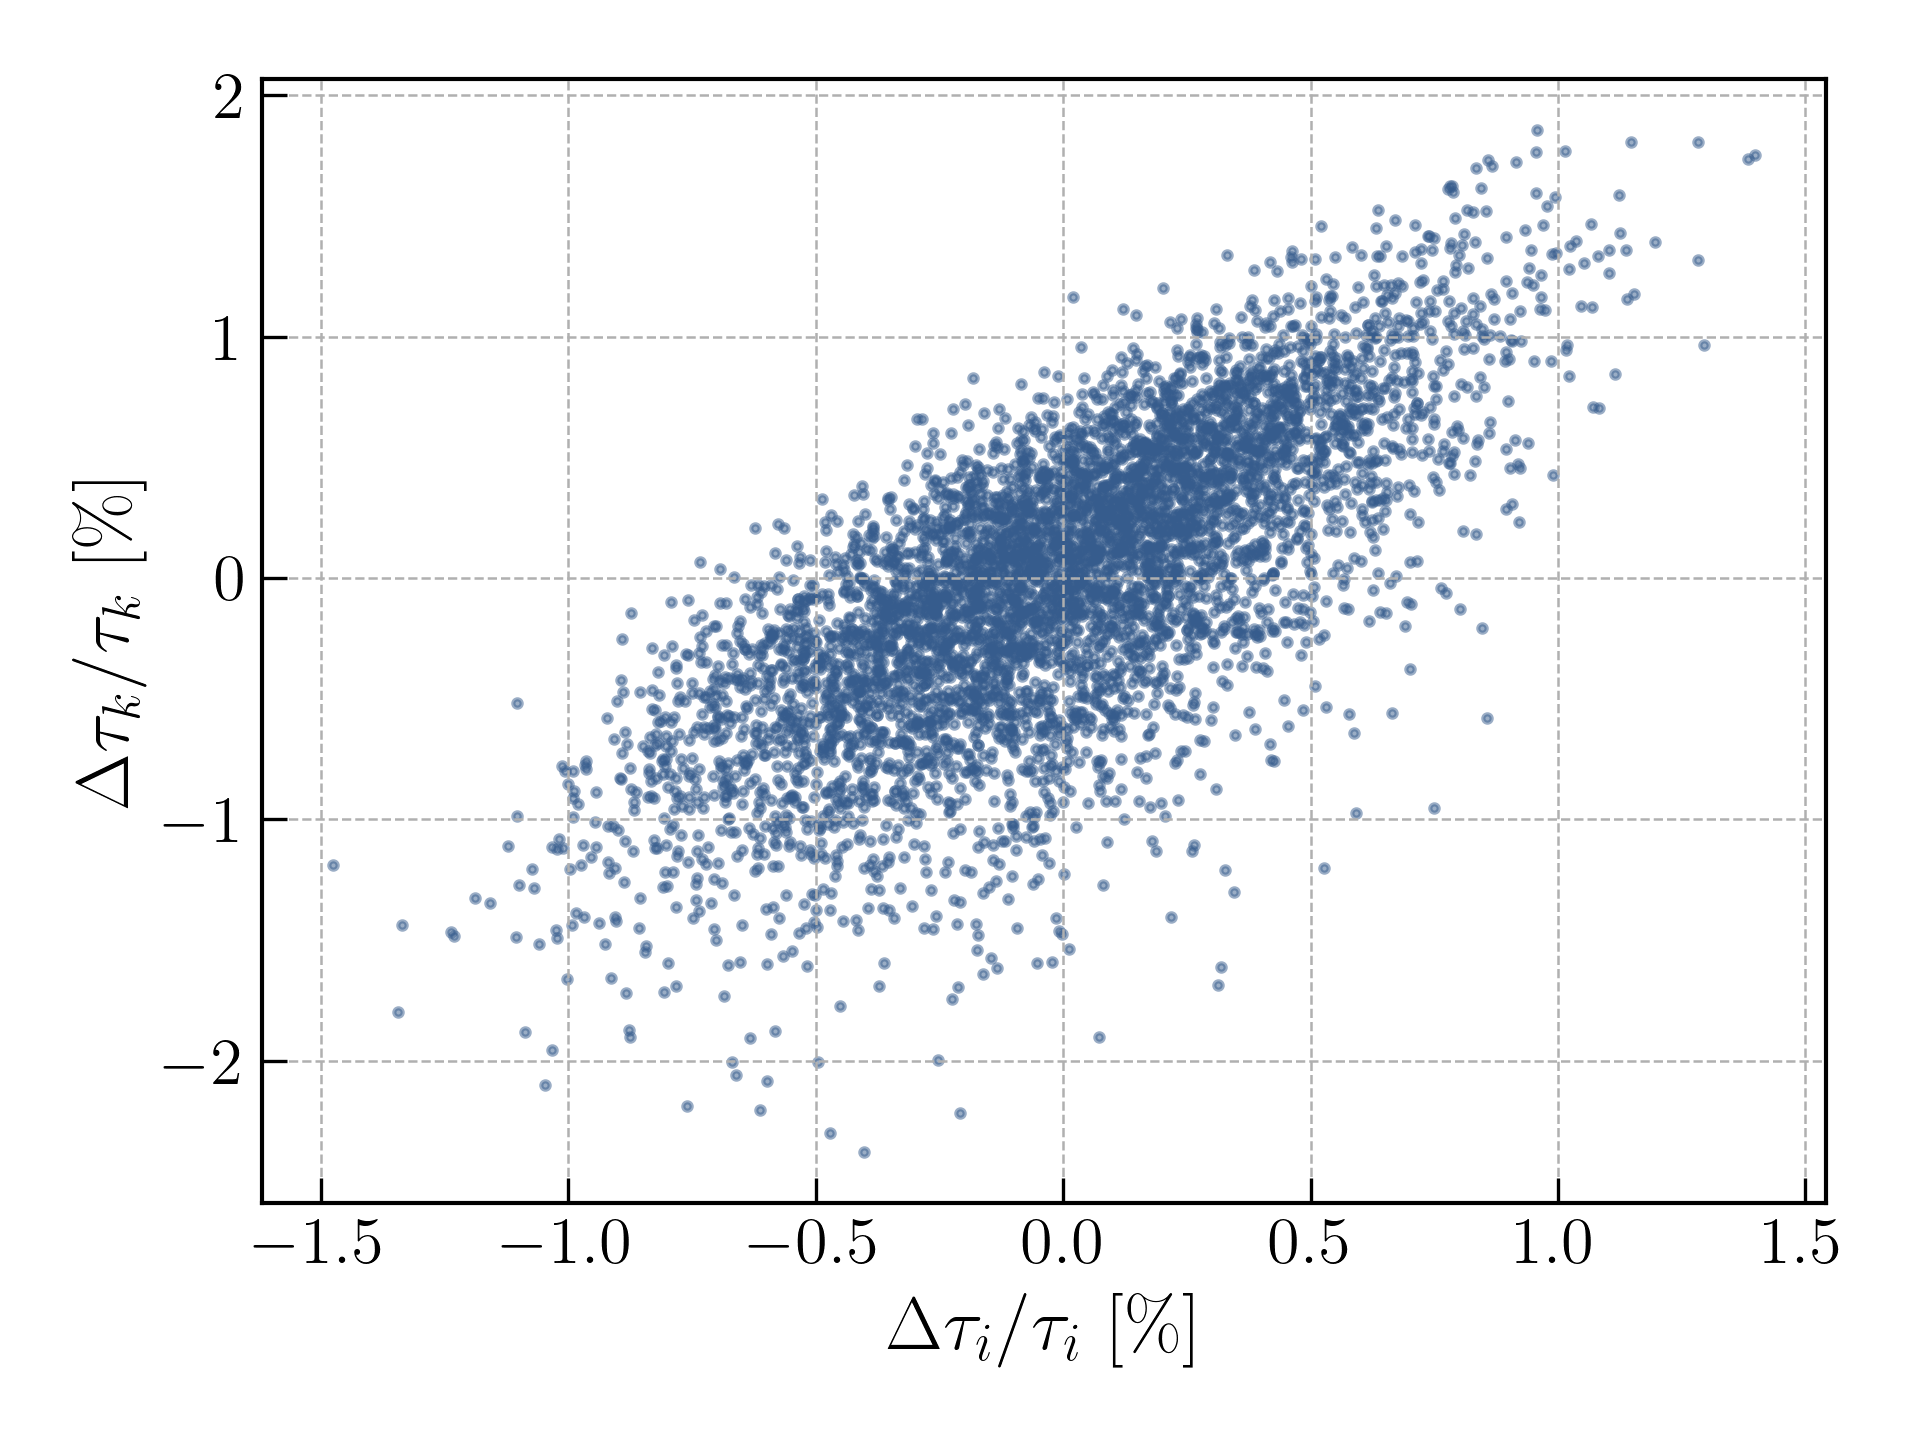
\includegraphics[width=0.45\linewidth]{images/iaea/sens_lam_halflife_I137_2.png}
}
\caption{These plots show the sensitivity of the \gls{DNP} group one and two half-lives to the $^{137}$I half-life. The group one half-life $\tau_1$ does not correlate with the $^{137}$I half-life, resulting in a sample distribution with no discernible slope. The group two half-life $\tau_2$ has a strong, positive linear correlation with the $^{137}$I half-life with a \gls{PCC} of 0.73. This indicates that changes to the $^{137}$I half-life will have greater effects on the group two half-life than the group one half-life.}
\label{fig:sens-iaea-jendl}
\end{figure}


Table \ref{tab:iaea-jendl5-yld-hl} shows how the total delayed neutron yield $\nu_d$ and average half-life $\bar{\tau}$ compares between the value from the $I$ \glspl{DNP} and the six \gls{DNP} groups.
The differences between both are well within the uncertainty bounds, indicating the six groups are sufficiently capturing the general behavior of the delayed neutrons.


\begin{table}[]
    \centering
    \caption{IAEA beta-delayed neutron emission database and JENDL-5 nuclear data delayed neutron yield and average half-life values.}
    \begin{tabular}{lrl}
        \hline
        Parameter & Value & Units\\
        \hline
        $\nu_d(I)$ & $0.0160 \pm 0.0009$ &$ [-]$\\
        $\nu_d(K)$ & $0.0160 \pm 0.0008$ & $[-]$\\
        $\Delta \nu_d$ & $0.0263 \pm 123$ & $[pcm]$\\
        \hline
        $\bar{\tau} (I)$ & $9.1 \pm 0.5$ & $[s]$\\
        $\bar{\tau} (K)$ & $9.0 \pm 0.4$ & $[s]$\\
        $\Delta \bar{\tau}$ & $0.01 \pm 0.7$ & $[s]$\\
        \hline
    \end{tabular}
    \label{tab:iaea-jendl5-yld-hl}
\end{table}

Table \ref{tab:iaea-jendl5-PCCi} shows the ten largest $PCC_i$ terms, which reveals which \glspl{DNP} have the greatest impact on the \gls{DNP} group parameters $\nu_{d,k}$ and $\tau_k$.
This table shows that bromine alone has five isotopes that strongly affect the \gls{DNP} group parameters, with $^{87}$Br being the dominant isotope due to its long-half life that makes it the primary \gls{DNP} for the group one parameters.
Generally, \glspl{DNP} will have a large $PCC_i$ for one of two reasons: they have a large delayed neutron yield and may affect several parameters moderately, such as $^{137}$I; or they have a half-life that causes them to have a large impact on one specific group, such as $^{87}$Br.

\begin{table}[]
    \centering
    \caption{IAEA beta-delayed neutron emission database and JENDL-5 nuclear data ten largest \glspl{PCC}.}
    \begin{tabular}{ll}
        \hline
       Nuclide & $PCC_{i}$ \\
       \hline
       $^{87}$Br & 3.678703 \\
       $^{88}$Br & 3.397623 \\
       $^{137}$I & 3.325644 \\
       $^{96}$Rb & 3.277932 \\
       $^{97}$Rb & 2.547497 \\
       $^{94}$Rb & 2.157988 \\
       $^{138}$I & 2.126428 \\
       $^{89}$Br & 2.111075 \\
       $^{90}$Br & 1.768819 \\
       $^{91}$Br & 1.670366 \\
        \hline
    \end{tabular}
    \label{tab:iaea-jendl5-PCCi}
\end{table}

Table \ref{tab:iaea-jendl5-Ui} shows the ten largest $U_i$ terms, which corresponds to which \glspl{DNP} have the largest uncertainties relative to their impact on the \gls{DNP} group parameters $\nu_{d,k}$ and $\tau_k$.
These ten \glspl{DNP} do not overlap at all with Table \ref{tab:iaea-jendl5-PCCi}, indicating that the JENDL-5 cumulative fission yields and IAEA beta-delayed neutron emission database have small relative uncertainties for the \glspl{DNP} in Table \ref{tab:iaea-jendl5-PCCi} as otherwise those \glspl{DNP} would dominate Table \ref{tab:iaea-jendl5-Ui}.
Interestingly, it appears that cobalt has several isotopes that have large $U_i$ values, indicating that element has large relative uncertainties in its nuclear data relative to its impact on the \gls{DNP} group parameters.

\begin{table}[]
    \centering
    \caption{IAEA beta-delayed neutron emission database and JENDL-5 nuclear data ten largest uncertainty-weighted \glspl{PCC}.}
    \begin{tabular}{ll}
        \hline
       Nuclide & $U_{i}$ \\
       \hline
       $^{105}$Zr & 0.281379 \\
       $^{72}$Co & 0.268531 \\
       $^{116}$Ru & 0.260299 \\
       $^{105}$Y & 0.246537 \\
       $^{75}$Co & 0.244795 \\
       $^{68}$Co & 0.235227 \\
       $^{116}$Rh & 0.231495 \\
       $^{71}$Co & 0.229786 \\
       $^{99}$Kr & 0.226118 \\
       $^{70}$Co & 0.222885 \\
        \hline
    \end{tabular}
    \label{tab:iaea-jendl5-Ui}
\end{table}

Figure \ref{fig:iaea-jendl-bar-uiv} gives a more detailed view on which \gls{DNP} values specifically lead to the large $U_i$ values.
This offers slightly more insight than Table \ref{tab:iaea-jendl5-Ui}, which sums over the various \gls{DNP} values.
This figure shows that the half-lives $\tau$ and emission probabilities $P_n$ are the primary drivers of $U_{i}$, at least for the ten most impactful \glspl{DNP}.
This indicates that the JENDL-5 cumulative fission yields offer sufficiently relative uncertainties compared to the relative uncertainties from the IAEA beta-delayed neutron emission database.


\begin{figure}
    \centering
    
\includegraphics[width=0.5\linewidth]{images/iaea/pcc-bar.png}
    \caption{The ten largest uncertainty-weighted \glspl{PCC} $U_{i,v}$ sorted by \gls{DNP} and associated \gls{DNP} value from JENDL-5 cumulative fission yields and IAEA beta-delayed neutron emission database half-lives and emission probabilities.}
    \label{fig:iaea-jendl-bar-uiv}
\end{figure}


Figure \ref{fig:pcc-charts-iaea-jendl} shows the $PCC_i$ and $U_i$ plotted on the chart of the nuclides.
These plots do not limit to only the top ten largest values, but instead show how all of the values compare among each other.
The values of $U_i$ are all smaller than those of $PCC_i$, because all of the relative uncertainties are less than 1.
There do not appear to be any clear trends, though in Figure \ref{fig:pcc-charts-iaea-jendl}(a), some horizontal bands of larger $PCC_i$ values can be seen for 35 protons, 37 protons, and 53 protons; these correspond to bromine, rubidium, and iodine, respectively.

\begin{figure}[!ht]
\centering
\subfloat[The $PCC_i$, or total \gls{PCC}, calculated for each \gls{DNP}.]{
  
\includegraphics[width=0.45\linewidth]{images/iaea/chart_PCC.png}
}
\hspace{0.05\linewidth}
\subfloat[The $U_i$, or total uncertainty-weighted \gls{PCC}, for each \gls{DNP}.]{
  
\includegraphics[width=0.45\linewidth]{images/iaea/chart_PCC_uncertainty.png}
}
\caption{Chart of nuclide plots showing the \glspl{PCC} and uncertainty-weighted \glspl{PCC} using JENDL-5 cumulative fission yields and IAEA beta-delayed neutron emission database emission probabilities and half-lives.}
\label{fig:pcc-charts-iaea-jendl}
\end{figure}


\FloatBarrier